\subsection{Расстояние и размеры}
\term{Астрономическая единица}~--- единица измерения расстояния в астрономии, 
равная большой полуоси орбиты Земли.\begin{equation}
	1~\au = 149\:597\:870\:700~\text{м} \simeq 1.5 \times 10^{11}~\text{м}
\end{equation}

\term{Годичный параллакс} ($\pi$) объекта~--- это угол, под которым видно 
орбиту Земли из окрестностей данного объекта. Применяется к объектам вне 
Солнечной системы. \begin{equation}
	\sin \pi = \frac{a_\oplus}{r},
	\label{eq:parallax-sin}	
\end{equation}
где $a_\oplus$~--- большая полуось орбиты Земли и $r$~--- расстояние до объекта 
имеют одинаковые единицы измерений. Учитывая малость угла $\pi$, можно заменить $\sin\pi$ на $\pi$ в \eqref{eq:parallax-sin}, получим \begin{equation}
	\pi = \frac{a_\oplus}{r}
	\label{eq:parallax}
\end{equation} 

\begin{figure}[h!]
\centering
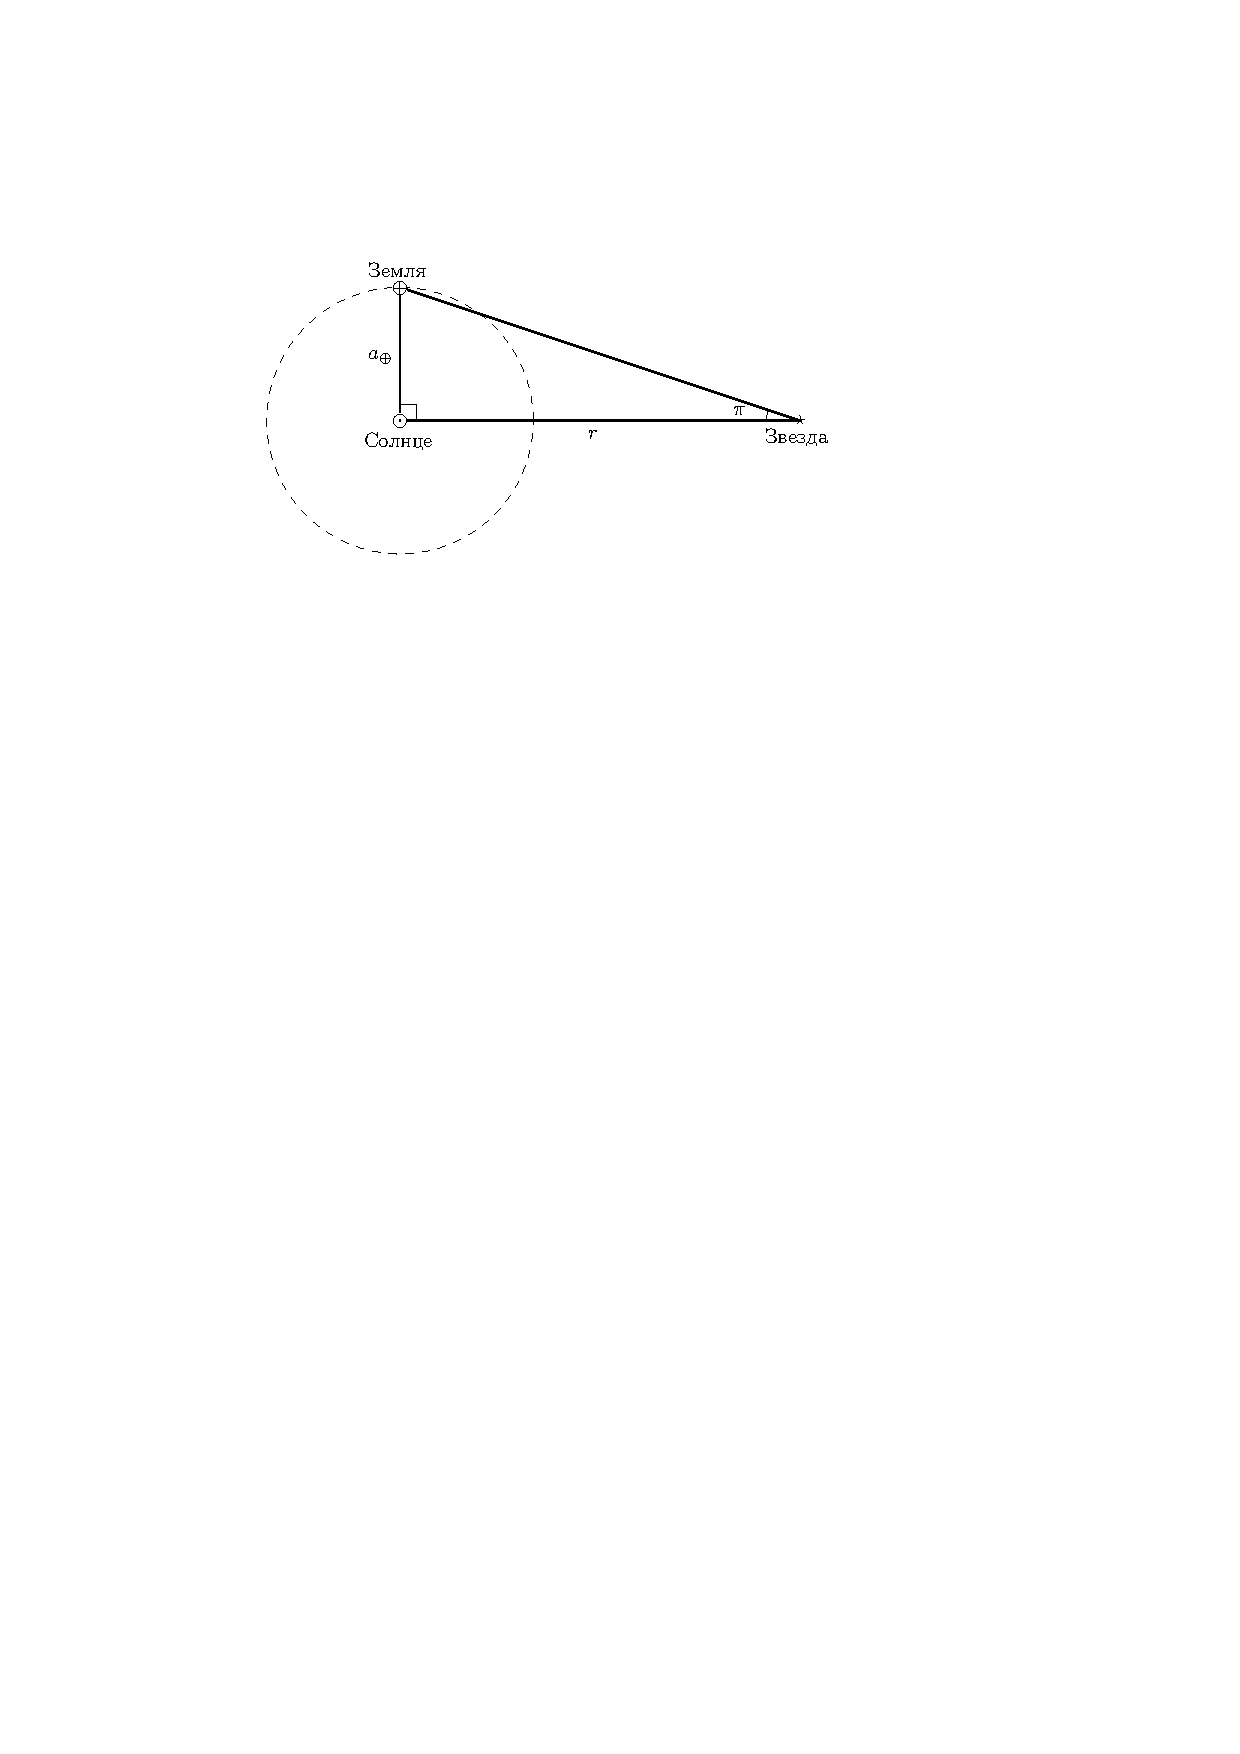
\includegraphics[width = 0.7\tw]{parallax.pdf}
\caption{Схема годичного параллакса}
\end{figure}

Расстояние $r$, с которого большая полуось орбиты Земли $a_\oplus$ видна под углом $\pi = 1''$ называется \term{1 парсеком}. Так как \begin{equation}
	1~\text{рад} = \frac{180^\circ}{\pi} \simeq  3 438' \simeq 206265'' 
\quad \Longrightarrow \quad \mathsf{1~\text{\sffamily пк} = 
206265~\text{\sffamily а.\,е.}},
\end{equation} 
следовательно, записывая большую полуось орбиты Земли в \au, а расстояние до звезды в парсеках, получаем параллакс в секундах. Таким образом имеем следующую формулу:\begin{equation}
	r_\text{пк} = \frac{1~\au}{\pi''},
\end{equation}
где $\pi''$ --- годичный параллакс объекта в секундах дуги.


\term{Угловой размер объекта}~--- это угол, под которым видно объект. Для астрономии наиболее актуален угловой размер сферически симметричных объектов, для которых угловой размер (диаметр) определяется, как
\begin{equation}
\rho = 2 \arcsin \frac{R}{r}, 
\end{equation}
где $R$~--- радиус объекта, а $r$~--- расстояние до него.

В случаем, когда $r$ много больше размера объекта $R$, то есть $r\gg R$, можно воспользоваться приближением для малых углов, тогда \begin{equation}
	\rho \simeq \frac{2 R}{r}.
\end{equation}

\begin{figure}[h!]
	\begin{minipage}[b]{0.49\tw}
		\centering
		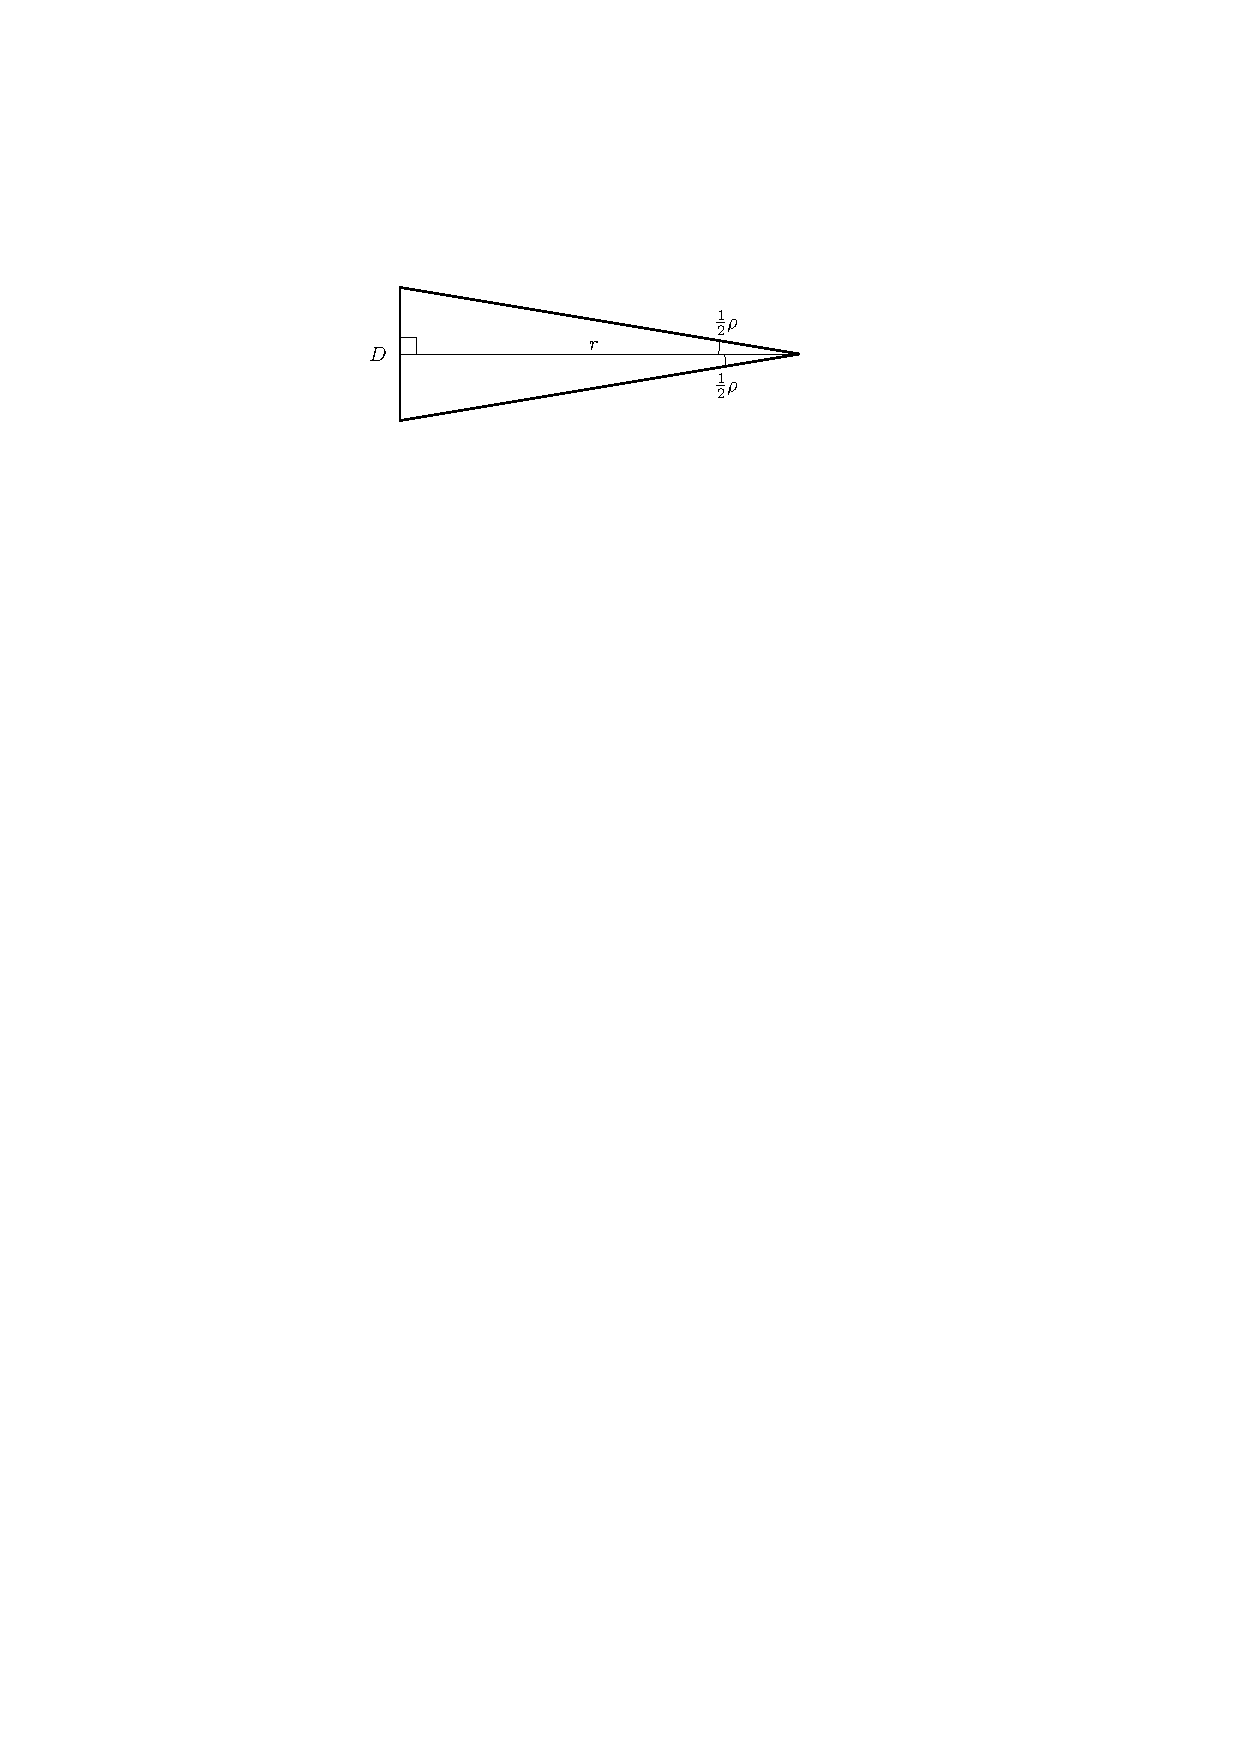
\includegraphics[width = 0.97\tw]{angle-size}
		\captionof{figure}{Угловой размер}
	\end{minipage}
	\hfill
	\begin{minipage}[b]{0.49\tw}
		\centering
		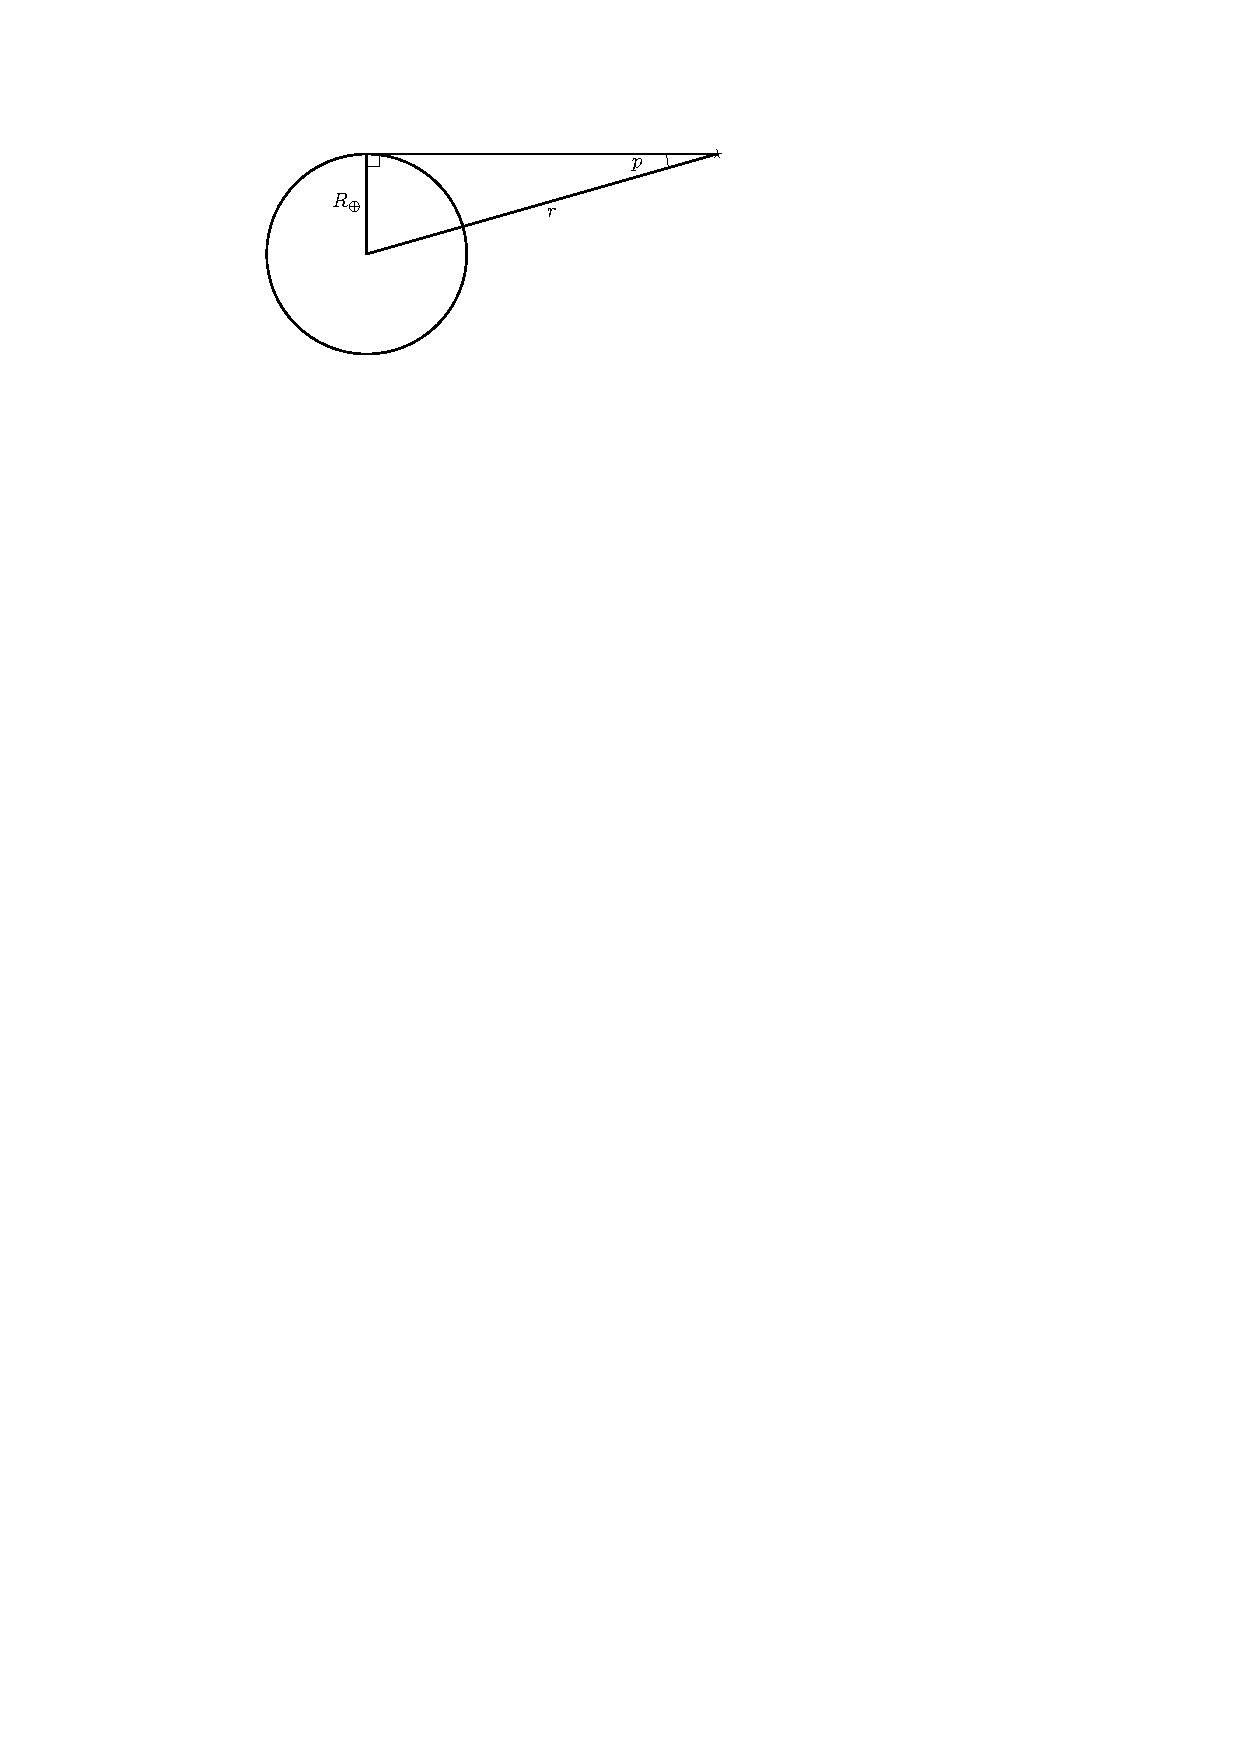
\includegraphics[width = 0.97\textwidth]{parallax-horiz}
		\captionof{figure}{Горизонтальный параллакс}
	\end{minipage}
\end{figure}

\term{Горизонтальный параллакс $(p)$}~--- это угол, под которым видно радиус Земли~$R_\oplus$, при положении светила на горизонте.
\begin{equation}
\sin p=\frac{R_\oplus}{r}.
\end{equation}

\term{Правило Тициуса-Боде} --- эмпирическая формула приблизительно описывающая 
радиусы орбит планет от Солнца:
\begin{equation}r=\frac{3\cdot 2^n+4}{10}, \quad n=-\infty, 0, 1, 2...
\end{equation}

